\chapter{Réalisation et résultats}

\section{Introduction}

Après avoir achevé l’étape d’analyse et conception de l’application, on va entamer dans ce chapitre la partie réalisation et implémentation dans laquelle on va s’assurer que le système est prêt pour être exploité par les utilisateurs finaux. Premièrement on choisit les technologies et puis on procède à la réalisation.


\section{Outils et technologies}

tech

python



\section{Interfaces graphiques}

\subsection{Interfaces de Finedge}

\begin{center}
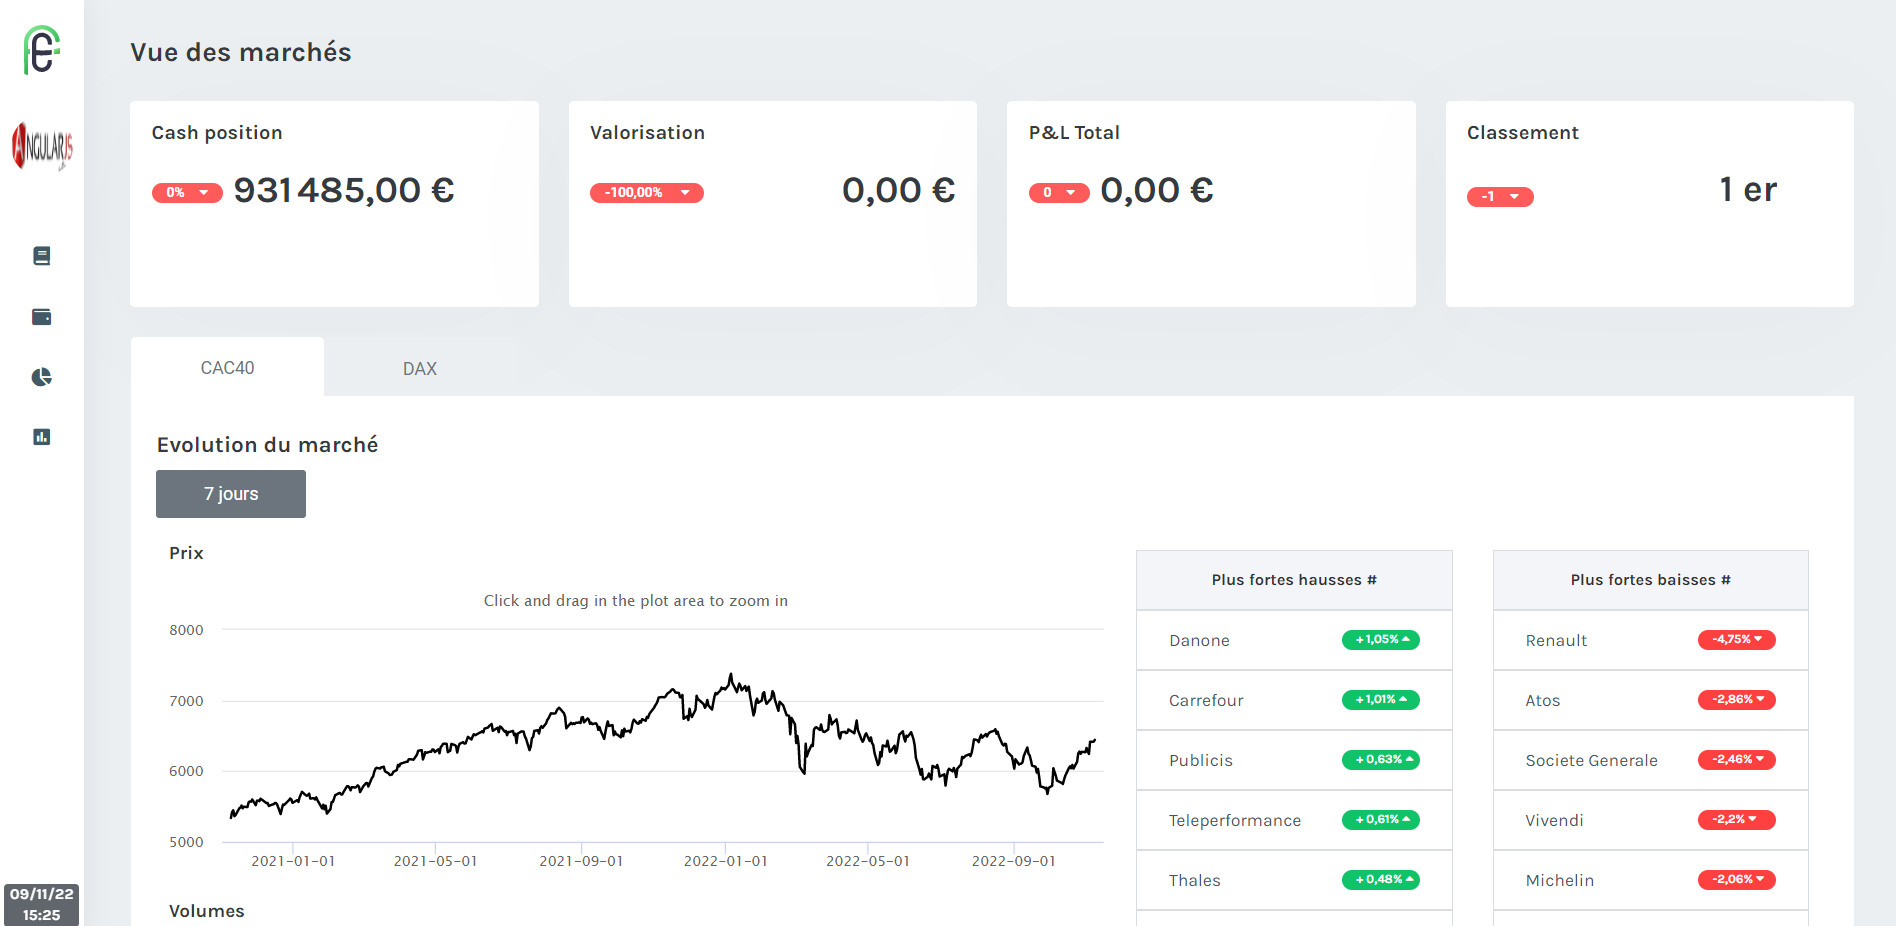
\includegraphics[scale=0.25]{images/fin} 
\end{center}


\begin{center}
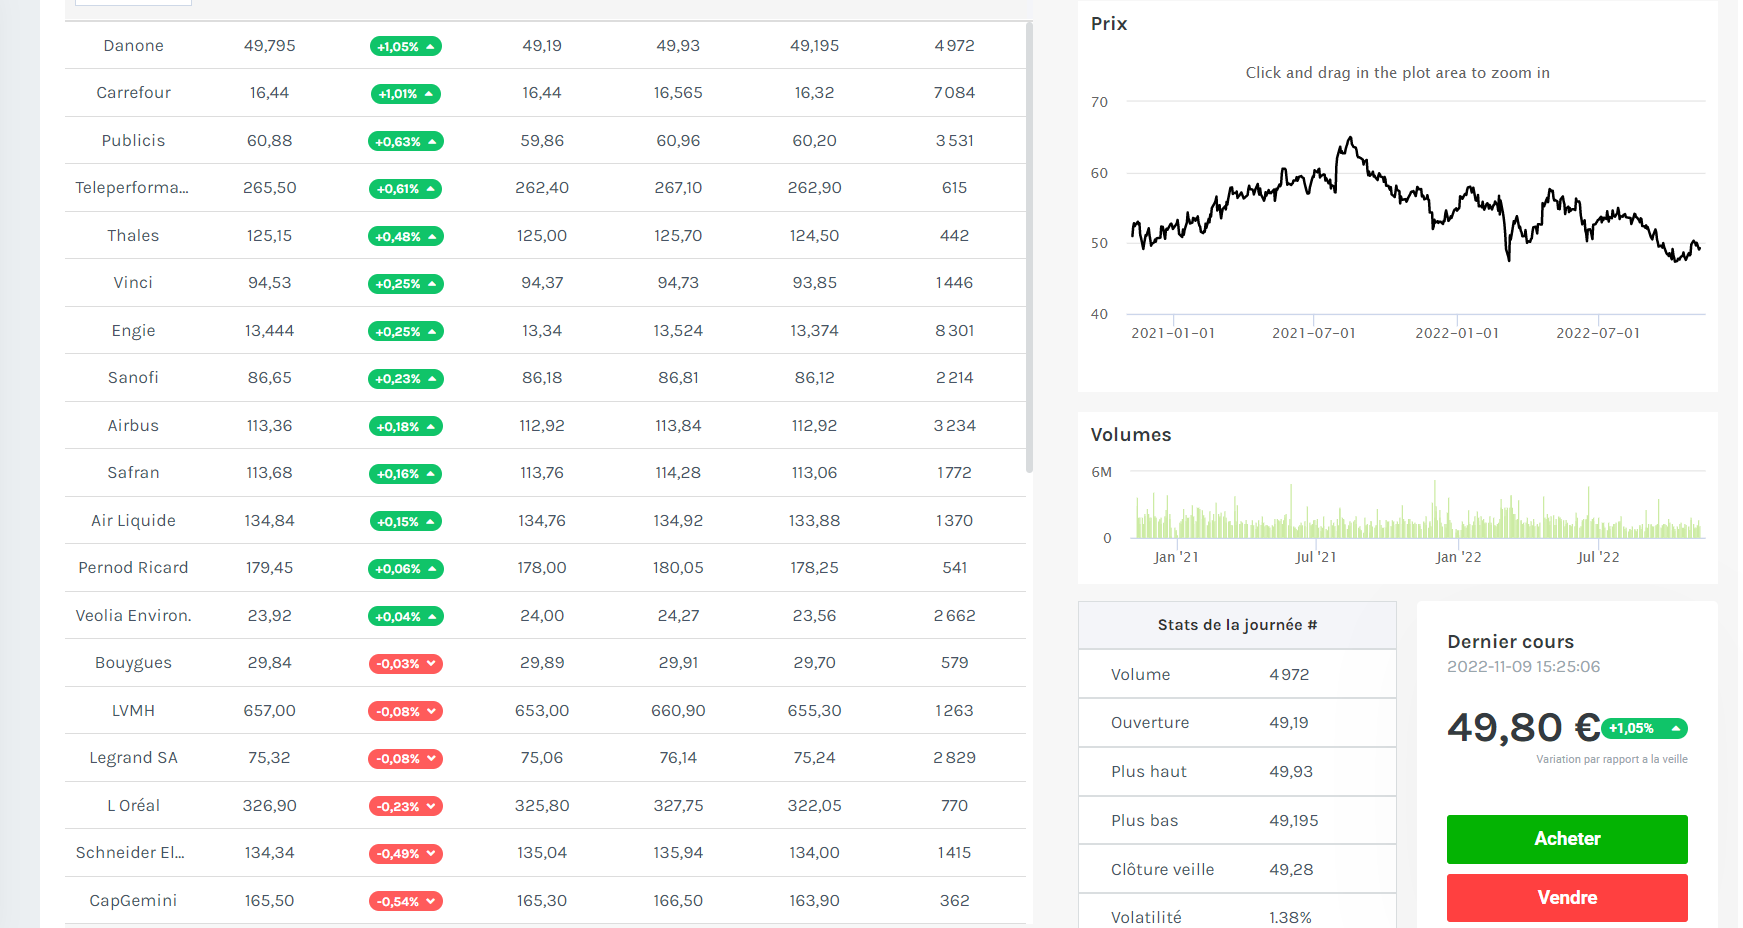
\includegraphics[scale=0.25]{images/fin2} 
\end{center}


\subsection{Interfaces de Pvgame}



\begin{center}
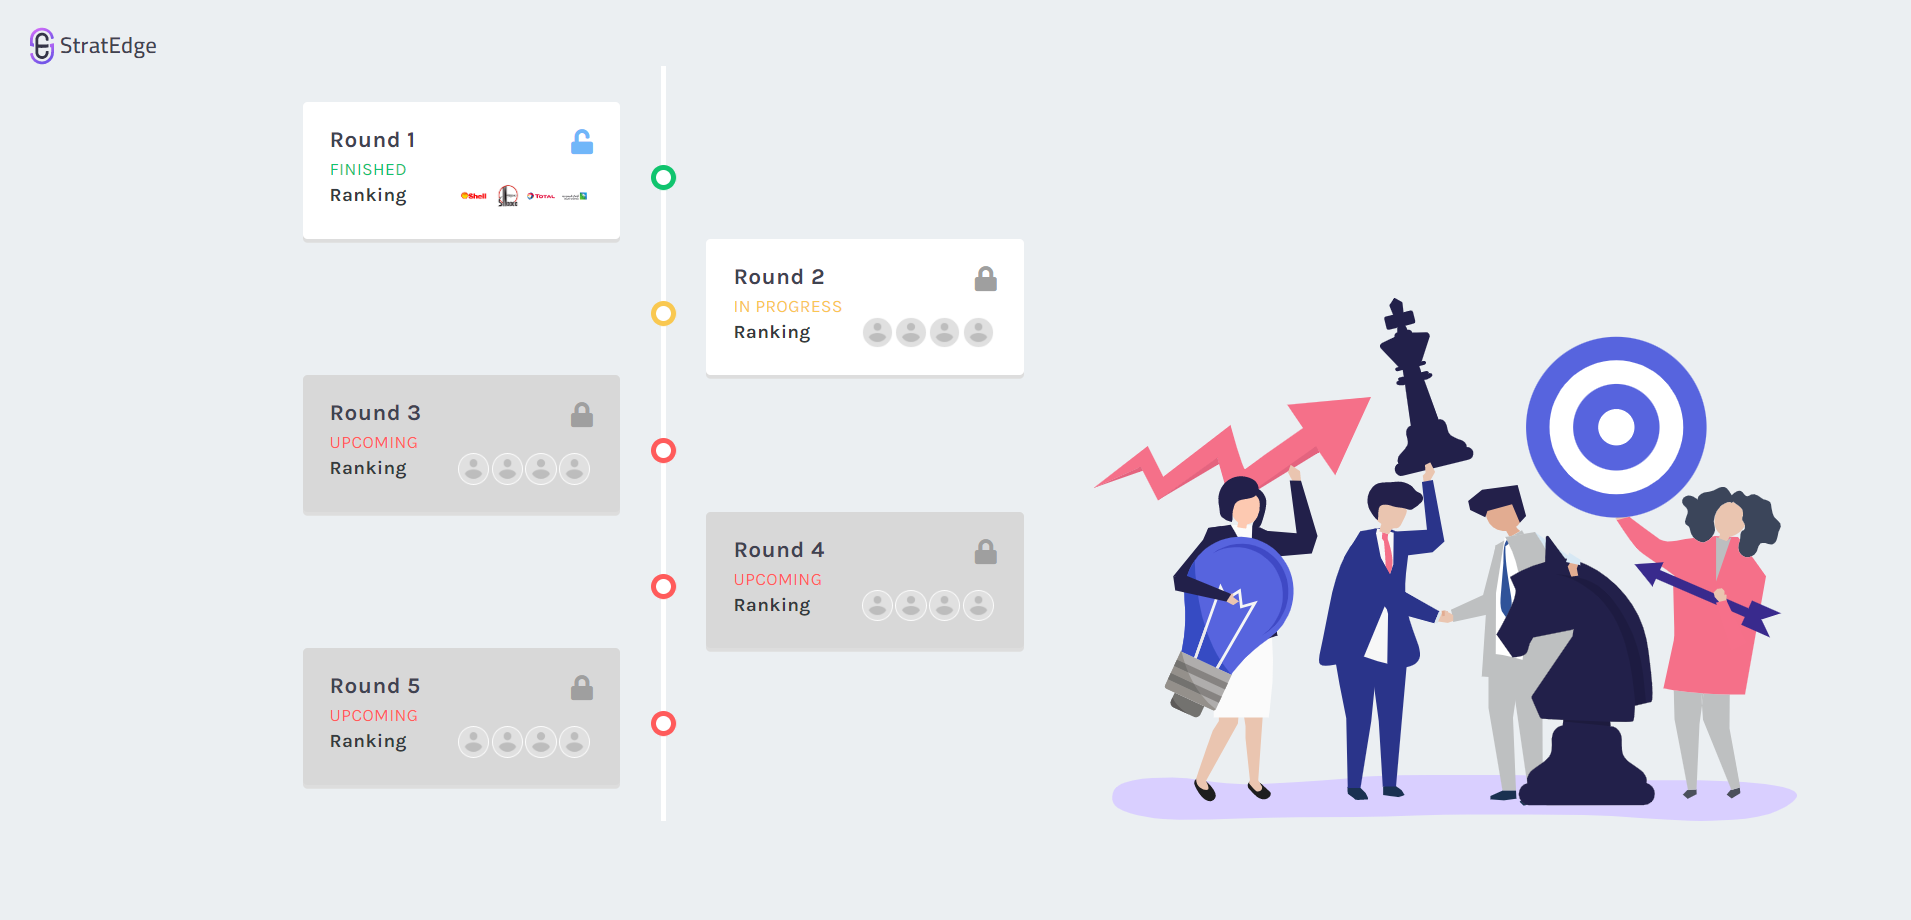
\includegraphics[scale=0.25]{images/strat} 
\end{center} 


\begin{center}
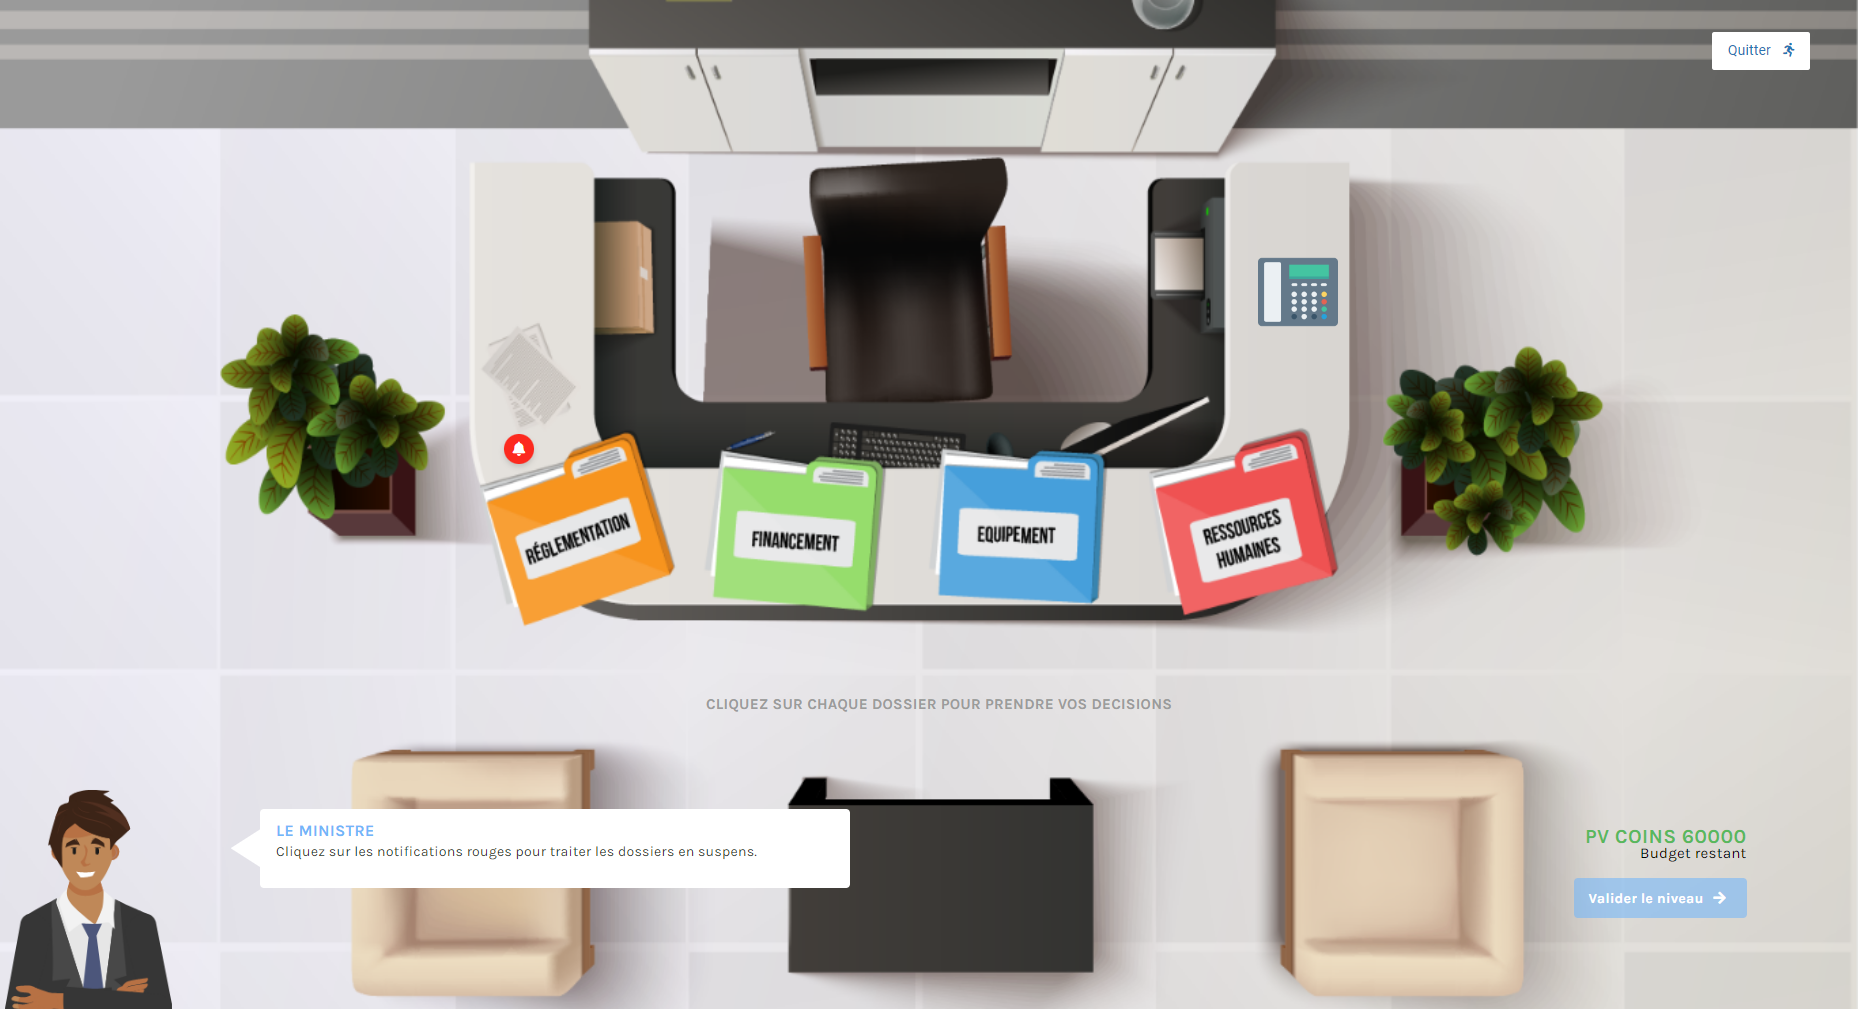
\includegraphics[scale=0.15]{images/1} 
\end{center} 




\begin{center}
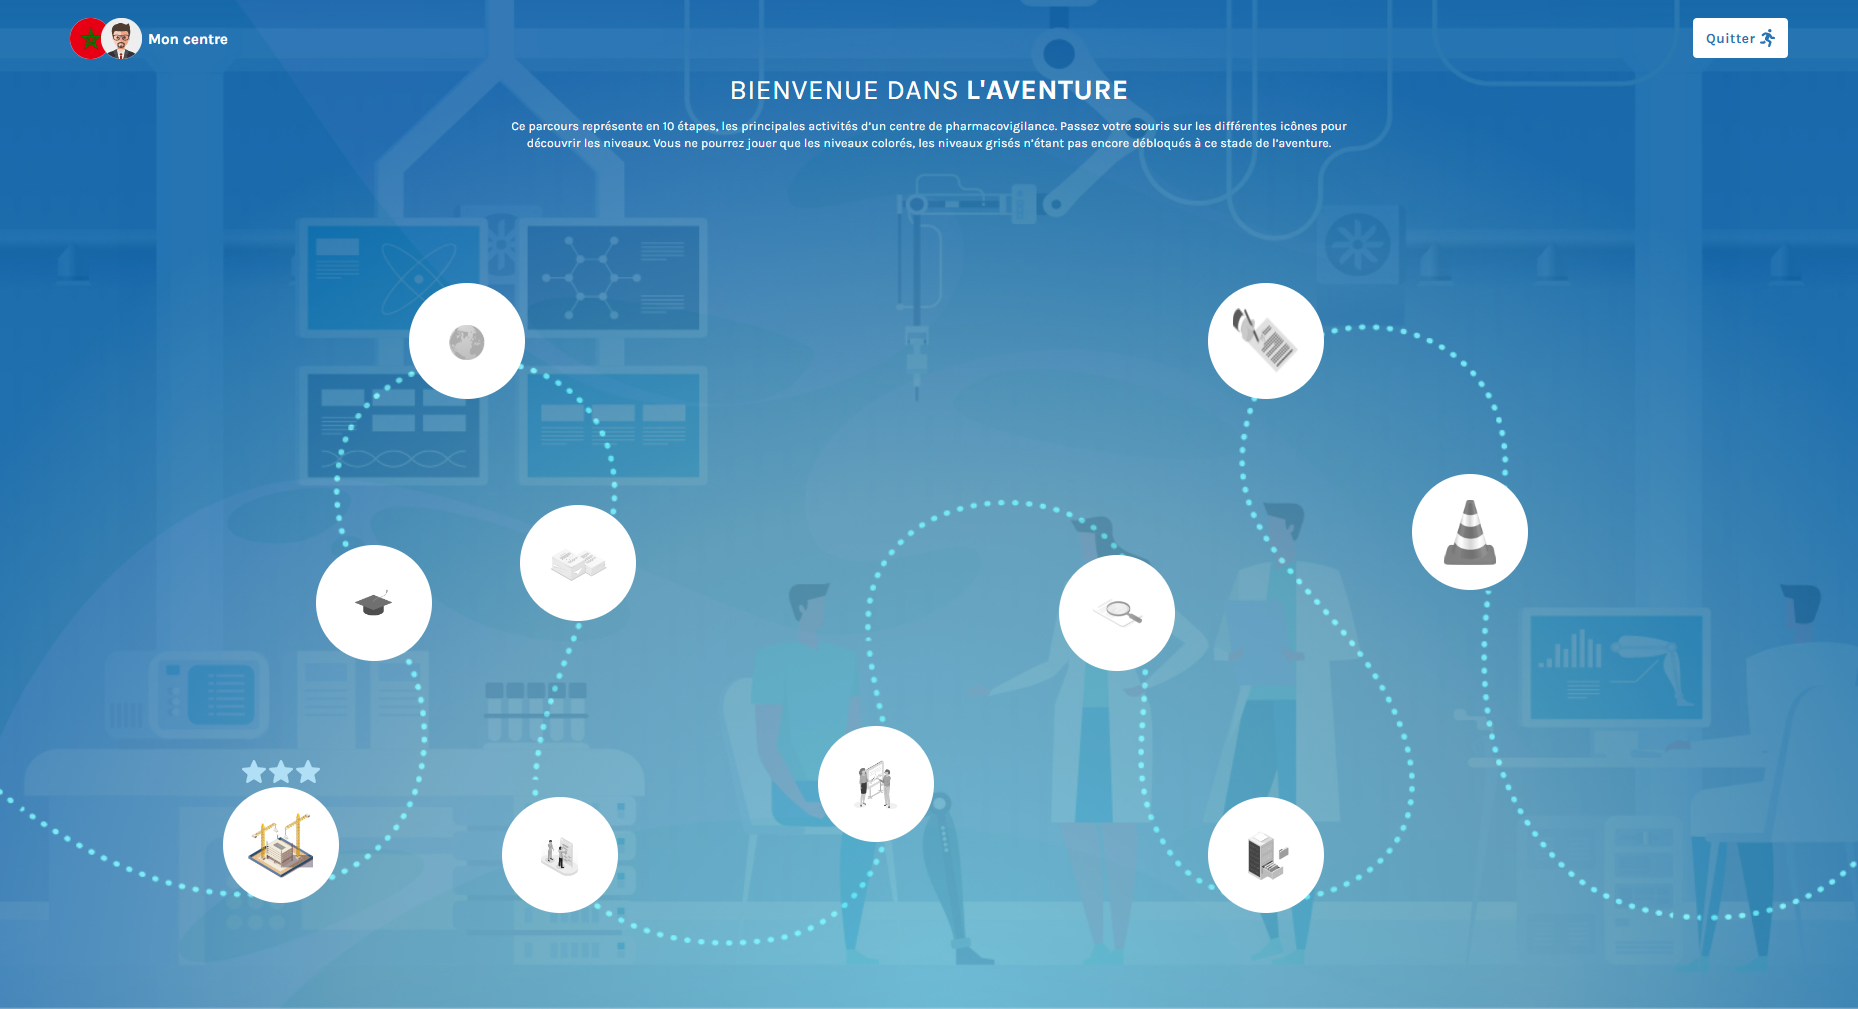
\includegraphics[scale=0.15]{images/2} 
\end{center}


\begin{center}
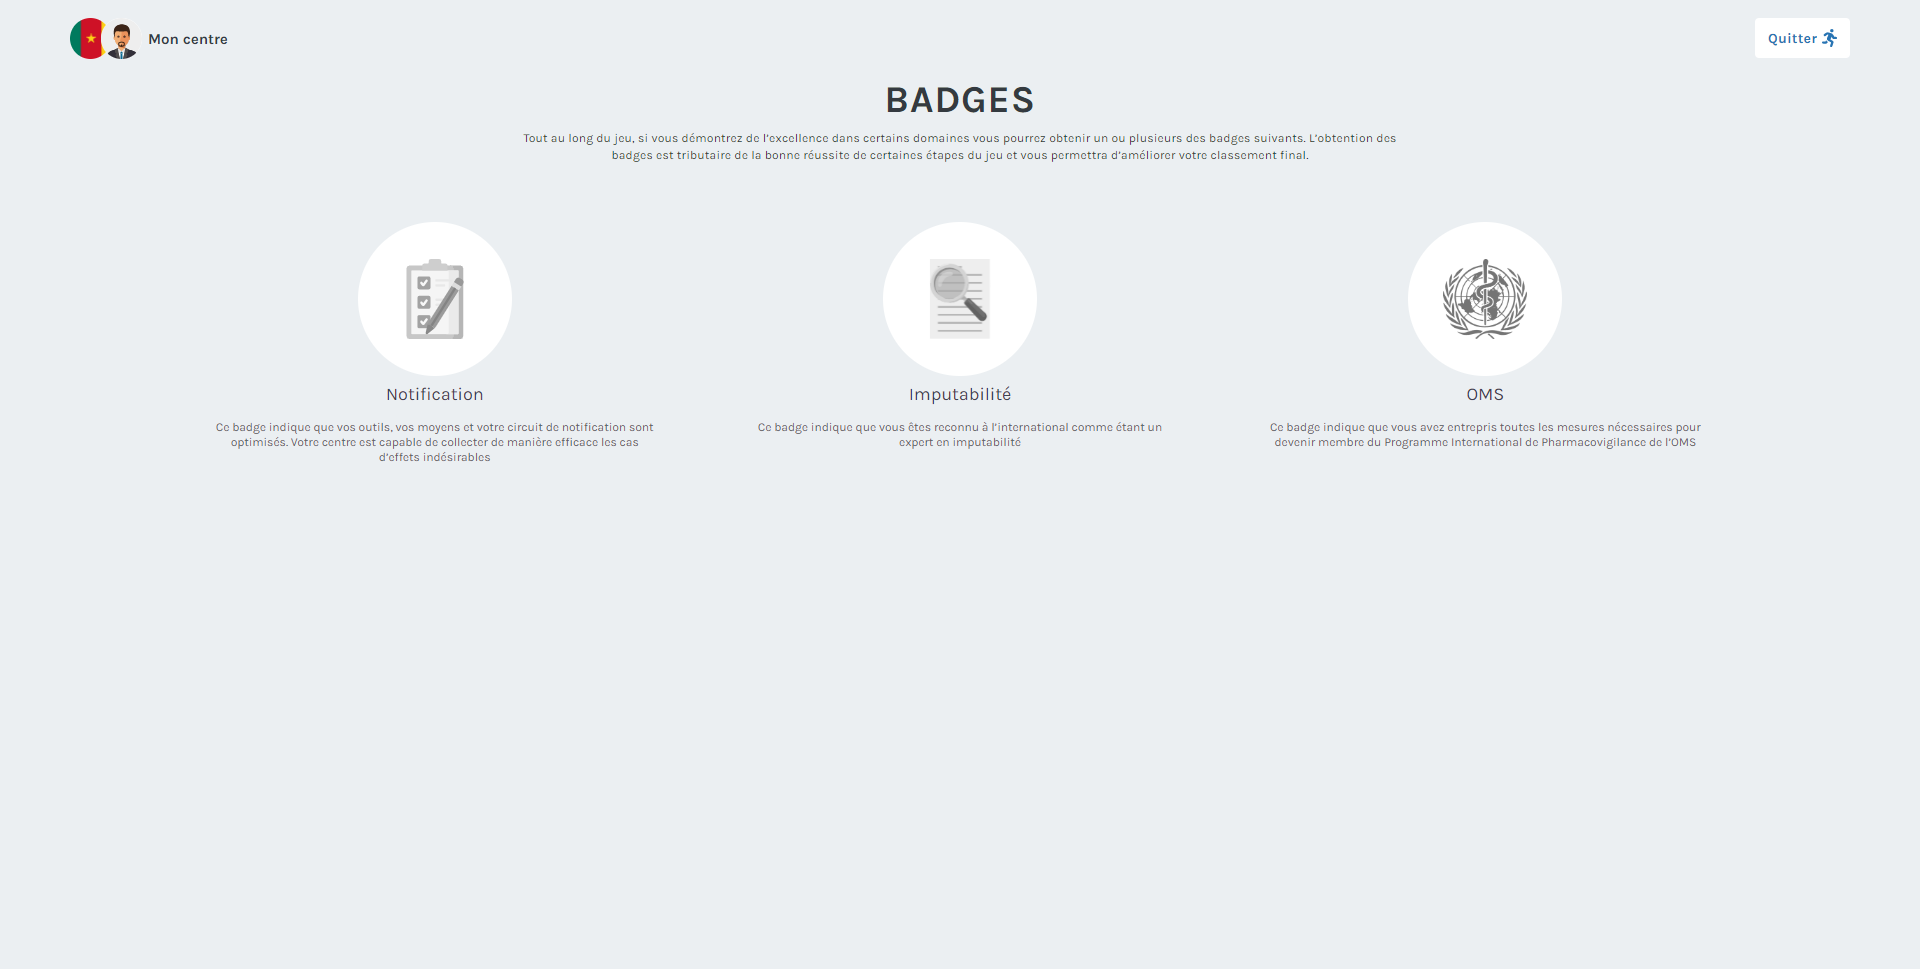
\includegraphics[scale=0.15]{images/5} 
\end{center}



\begin{center}
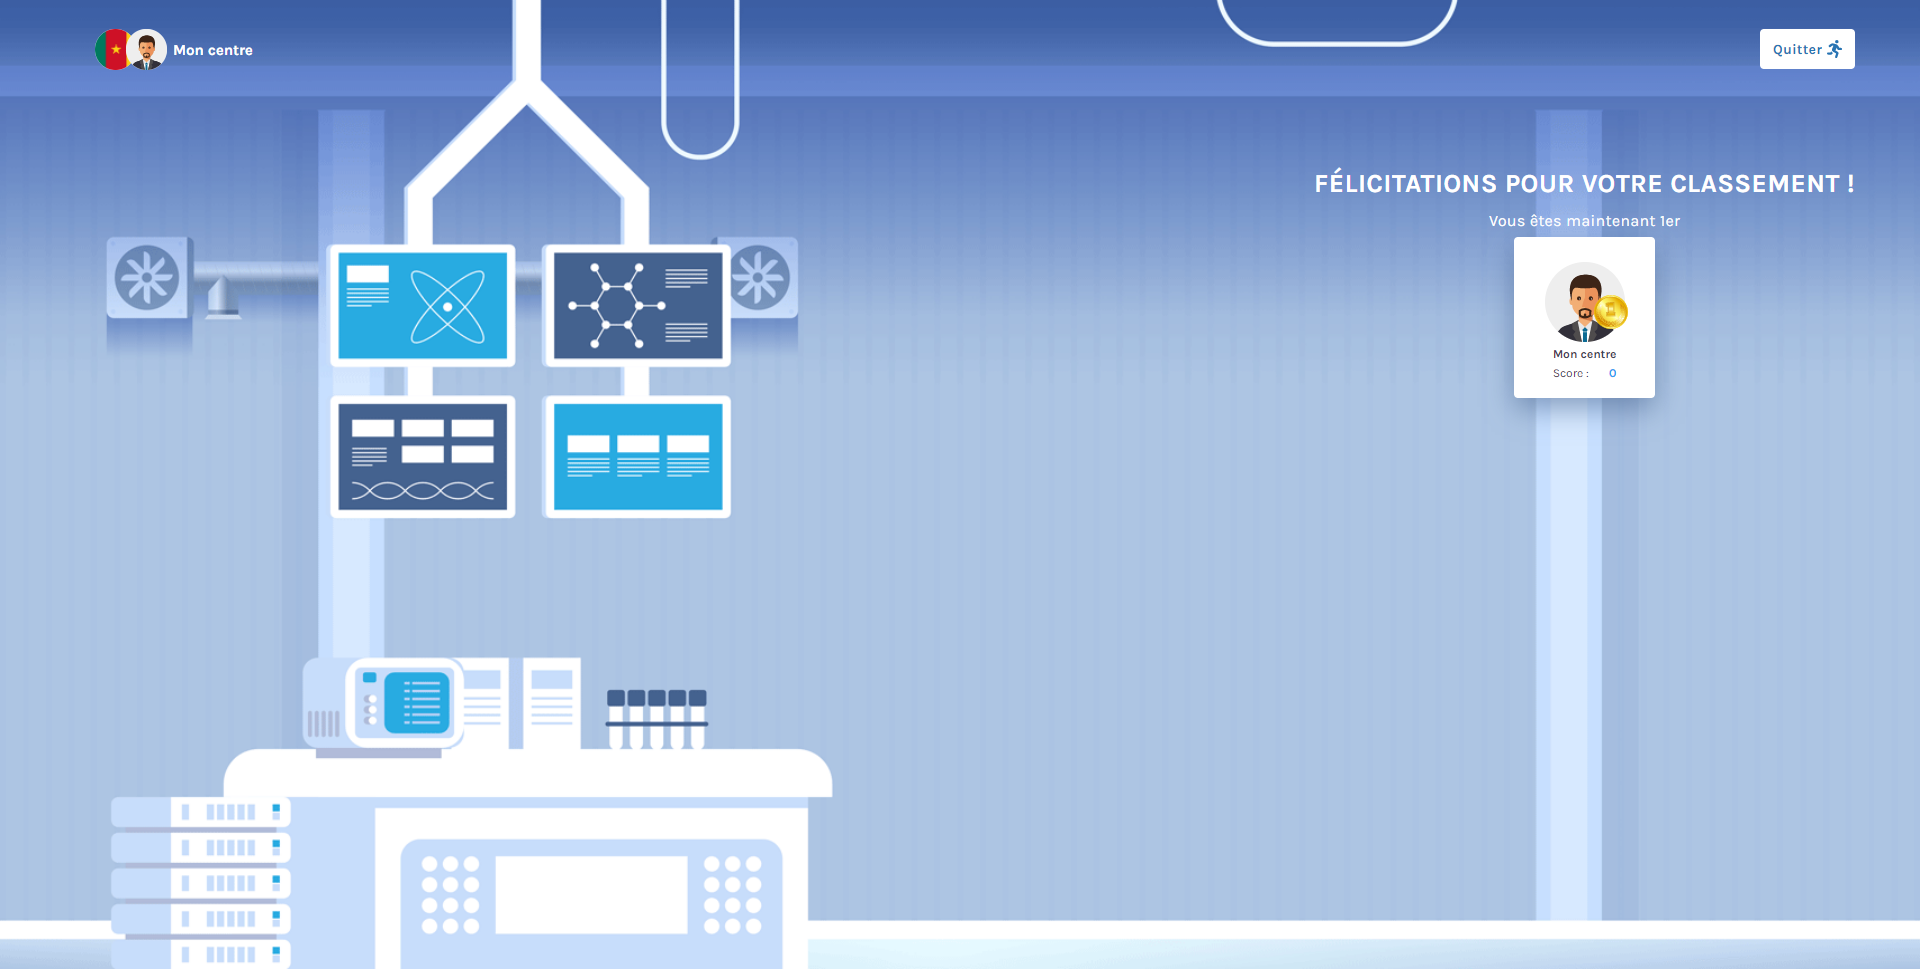
\includegraphics[scale=0.15]{images/4} 
\end{center}


\begin{center}
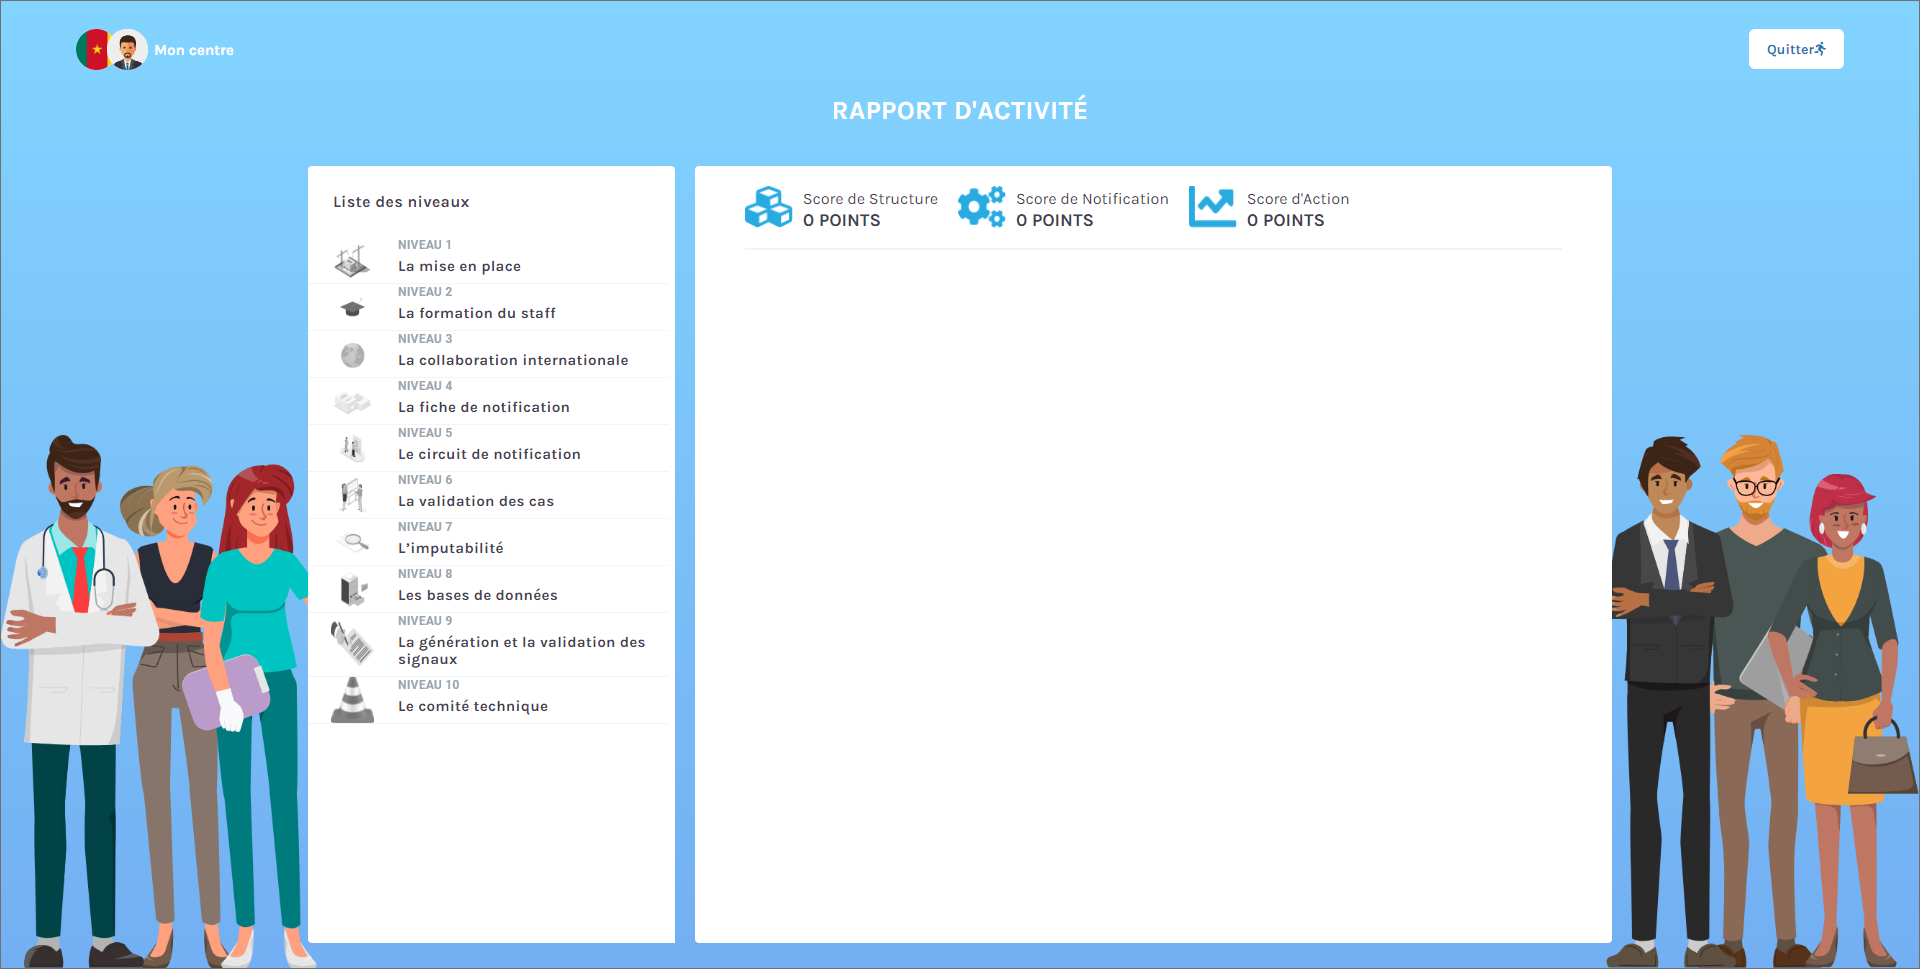
\includegraphics[scale=0.12]{images/3} 
\end{center}




\begin{center}
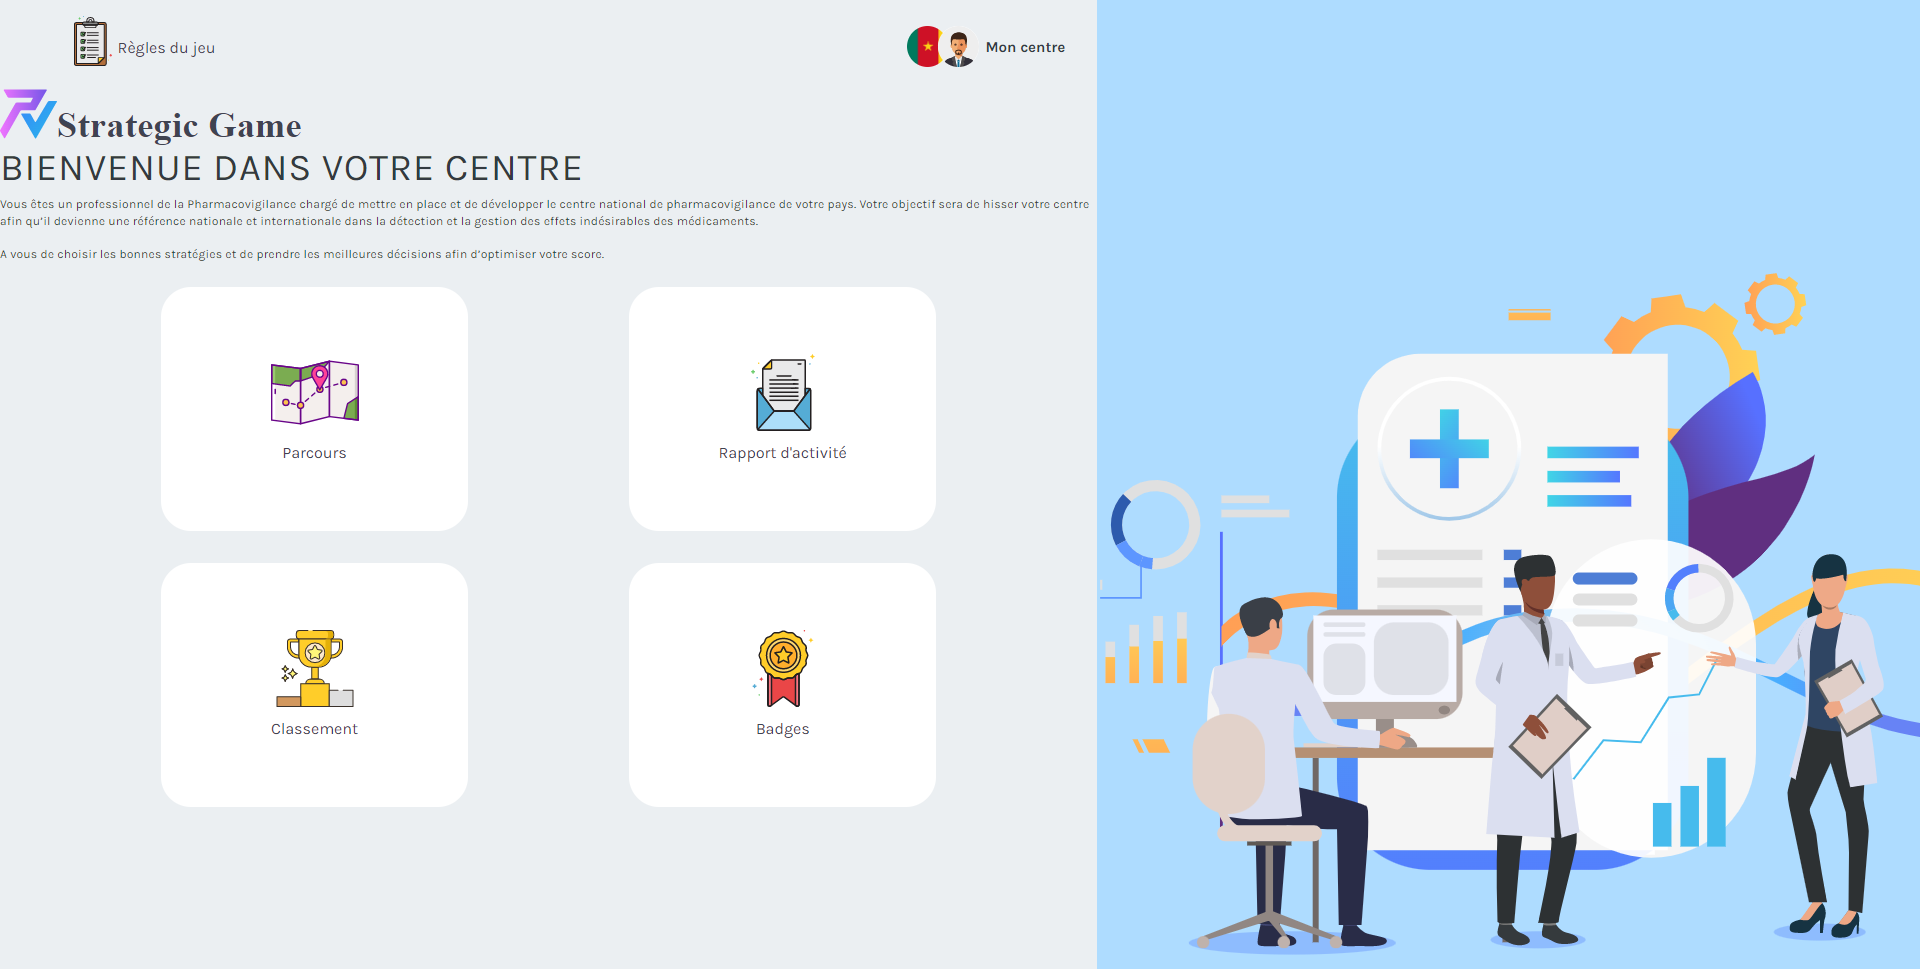
\includegraphics[scale=0.15]{images/6} 
\end{center}



\section{Conclusion}
La terminaison de cette étape marque la fin de notre projet, il reste à voir le résultat réél de ce projet et en tirer des conclusions, et puis voir des améliorations possible en guise de perspective.

